\documentclass[10pt]{article}

\usepackage{spheric}
%%%TITLE
\title{Three-Dimensional Sloshing Simulations by Using GPU-based MPS Method}
\date{}

%%AFFILIATIONS

\author[$\relax$]{Xiang Chen}
\author[$\relax$]{Xiao Wen}
\author[$\relax$]{Decheng Wan$^\dagger$}

\affil[$\relax$]{State Key Laboratory of Ocean Engineering, School of Naval Architecture, Ocean and Civil Engineering, Shanghai Jiao Tong University, Collaborative Innovation Center for Advanced Ship and Deep-Sea Exploration, Shanghai 200240, China}
\affil[$\relax$]{\email{\dagger}{dcwan@sjtu.edu.cn}}


%%DOCUMENT
\begin{document}

\maketitle

%\SelectedTopics{}

%%PLEASE PUT YOUR ABSTRACT HERE
\begin{abstract}
The liquid sloshing is a complicated and nonlinear phenomenon in a partially filled tank under external excitations, which will destroy the structure of tank walls and the stability of the movement. The moving particle semi-implicit method (MPS) is a Lagrangian particle method. Because the flow field is presented by particles that contain the information of mass, velocity and so on, MPS method can simulate flow with large deformation and nonlinear fragmentation of free surface effectively.

However, MPS suffers from high computation cost with the increase of particle number. This significantly limits its applications in 3D flows which include a large number of particles. The GPU (Graphics Processing Unit) is a multi-processor designed to optimize for the execution of massive number of threads. Therefore, GPU is a better choice for high parallel MPS method. Based on modified MPS, our group developed MPS-GPU-SJTU solver by using GPU acceleration. 

It is well known that the most computation time of MPS is consumed to solve PPE. One optimization strategy to reduce the storage and computation time of PPE is introduced. In addition, the convergent validation is carried out to verify the accuracy of GPU solver. And the 3-D sloshing problems are simulated by GPU and CPU solvers at the same time. The numerical impact pressure on tank walls is agreeable with experimental data. Nonlinear deformation of free surface, such as breaking wave, splashing, hitting the roof of tank and so on, can be observed. And it is also shown that the results of GPU solver show a good agreement with CPU and a large amount of computation time is reduced by GPU.

\begin{figure}[!htb]
\begin{minipage}[b]{0.46\linewidth}
\centering
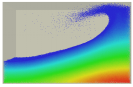
\includegraphics[width=0.45\textwidth]{16-11.png}~~
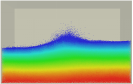
\includegraphics[width=0.45\textwidth]{16-12.png}
\caption{The flow fields of CPU}\label{fig:16-1}
\end{minipage}
\begin{minipage}[b]{0.05\linewidth}
~
\end{minipage}
\begin{minipage}[b]{0.46\linewidth}
\centering
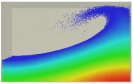
\includegraphics[width=0.45\textwidth]{16-21.png}~~
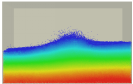
\includegraphics[width=0.45\textwidth]{16-22.png}
\caption{The flow fields of GPU}\label{fig:16-2}
\end{minipage}
\end{figure}

\end{abstract}


%%THE END OF ABSTRACT

\addbib

\end{document}
